\chapter{Literature Review}
\label{chap:literature}

\section {Overview}
\label{sec:overview}

With the widespread popularity of portable digital input devices like smartphones and tablets, there is increasing interest in the development of systems that can automatically interpret and convert paper based graphical information into an equivalent digital representation. This conversion to digital representations has been a topic of active research throughout the last decade \cite{Cordella_2000} \cite{Delalandre_2012}. \\

A fundamental way in which we communicate information, especially technical information, is through the use of diagrams \cite{Ouyang_2009}. Much of this effort is focused on the automatic conversion of manually sketched work / diagrams to a digital format which can be understood by CAD systems in order to be included into other larger bodies of work. \\

A key issue, at the heart of such research efforts, is the recognition of domain dependant symbols using domain-independent techniques. Authors commonly develop ad-hoc techniques which are difficult to reuse in other domains \cite{Llados}. Various approaches have been proposed to solve this issue, however challenges remain in terms of finding a general and efficient method which can be applied across domains with well establish performance and recognition accuracy. \\ 


In this literature review we direct our focus on the recognition of symbols from the electrical engineering and architectural domains. The main goal is to explain the process of symbol recognition in detail and then to highlight the different approaches adopted to-date to solve the problem of symbol recognition. \\


\section{What Is a Symbol?}
\label{sec:whatis}
The oxford dictionary defines the word 'symbol' as a mark or character which is used as a conventional representation of an object, function or process. In a very general way, a symbol can be defined as a contextually meaningful graphical shape of a specific application domain \cite{Llados}. Depending on the application, we can find various kinds of symbols in different industry fields like architecture, cartography, 
electronics, engineering etc. Each field use domain-dependant notations to construct their symbol designs. \\

In technical fields such as in architecture and engineering, symbols are designed in 2-dimensions (2D) using domain dependant notation \cite{Llados}.Simple symbols can be binary, made out of sets of line segments, both straight and in loops, such as electrical or architectural symbols , Fig. \ref{fig:electrical}. Symbols can also be complex, involving different levels of colours and shades, such as company logos \cite{Cordella_2000}, Fig. \ref{fig:logo}. \\

\begin{figure*}[h]
        \centering
        \begin{subfigure}[b]{0.4\textwidth}
                \centering
                \includegraphics[width=0.5\textwidth]{figures/introduction/electricalsymbol.jpg}
                \caption{}
                \label{fig:electrical}
        \end{subfigure}
        \begin{subfigure}[b]{0.4\textwidth}
                \centering
                \includegraphics[width=0.5\textwidth]{figures/introduction/logosymbol.jpg}
                \caption{}
                \label{fig:logo}
        \end{subfigure}
        \caption[Example of Symbols]{(a) An example of a contour based symbol and (b) An example of a complex symbol}
        \label{fig:symbolexamples}
\end{figure*}

From a symbol recognition stand point, documents of interest which mostly hold the most symbols can be grouped into three main categories \cite{Cordella_2000} :-

    \begin{enumerate}
        \item Technical drawings, such as flow diagrams and electrical schematics, Fig \ref{fig:electrical}
        \item Maps, topographical or geographical, Fig \ref{fig:map}
        \item Others, such as musical glyphs, Fig \ref{fig:score}
    \end{enumerate}

Symbols in such documents are formed depending on various domain dependent rules\cite{Cordella_2000}. Furthermore, when presented, they can contain added noise, be deformed, incomplete, and/or geometrically transformed. Symbols may also appear in isolation or in complex backgrounds. They may be in close proximity, touching or partially overlap each other. \\

\begin{figure*}[h]
\centering
    \begin{subfigure}[b]{0.4\textwidth}
        \centering
        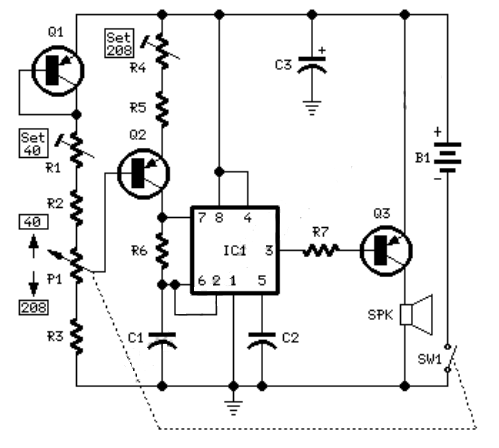
\includegraphics[width=1\textwidth]{figures/LitreatureReview/schematic.png}
        \caption{}
        \label{fig:electrical}
    \end{subfigure}
    \begin{subfigure}[b]{0.4\textwidth}
        \centering
        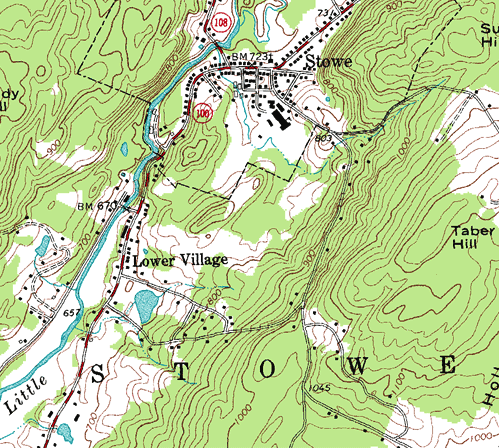
\includegraphics[width=1\textwidth]{figures/LitreatureReview/map2.png}
        \caption{}
        \label{fig:map}
    \end{subfigure}
        \begin{subfigure}[b]{0.4\textwidth}
        \centering
        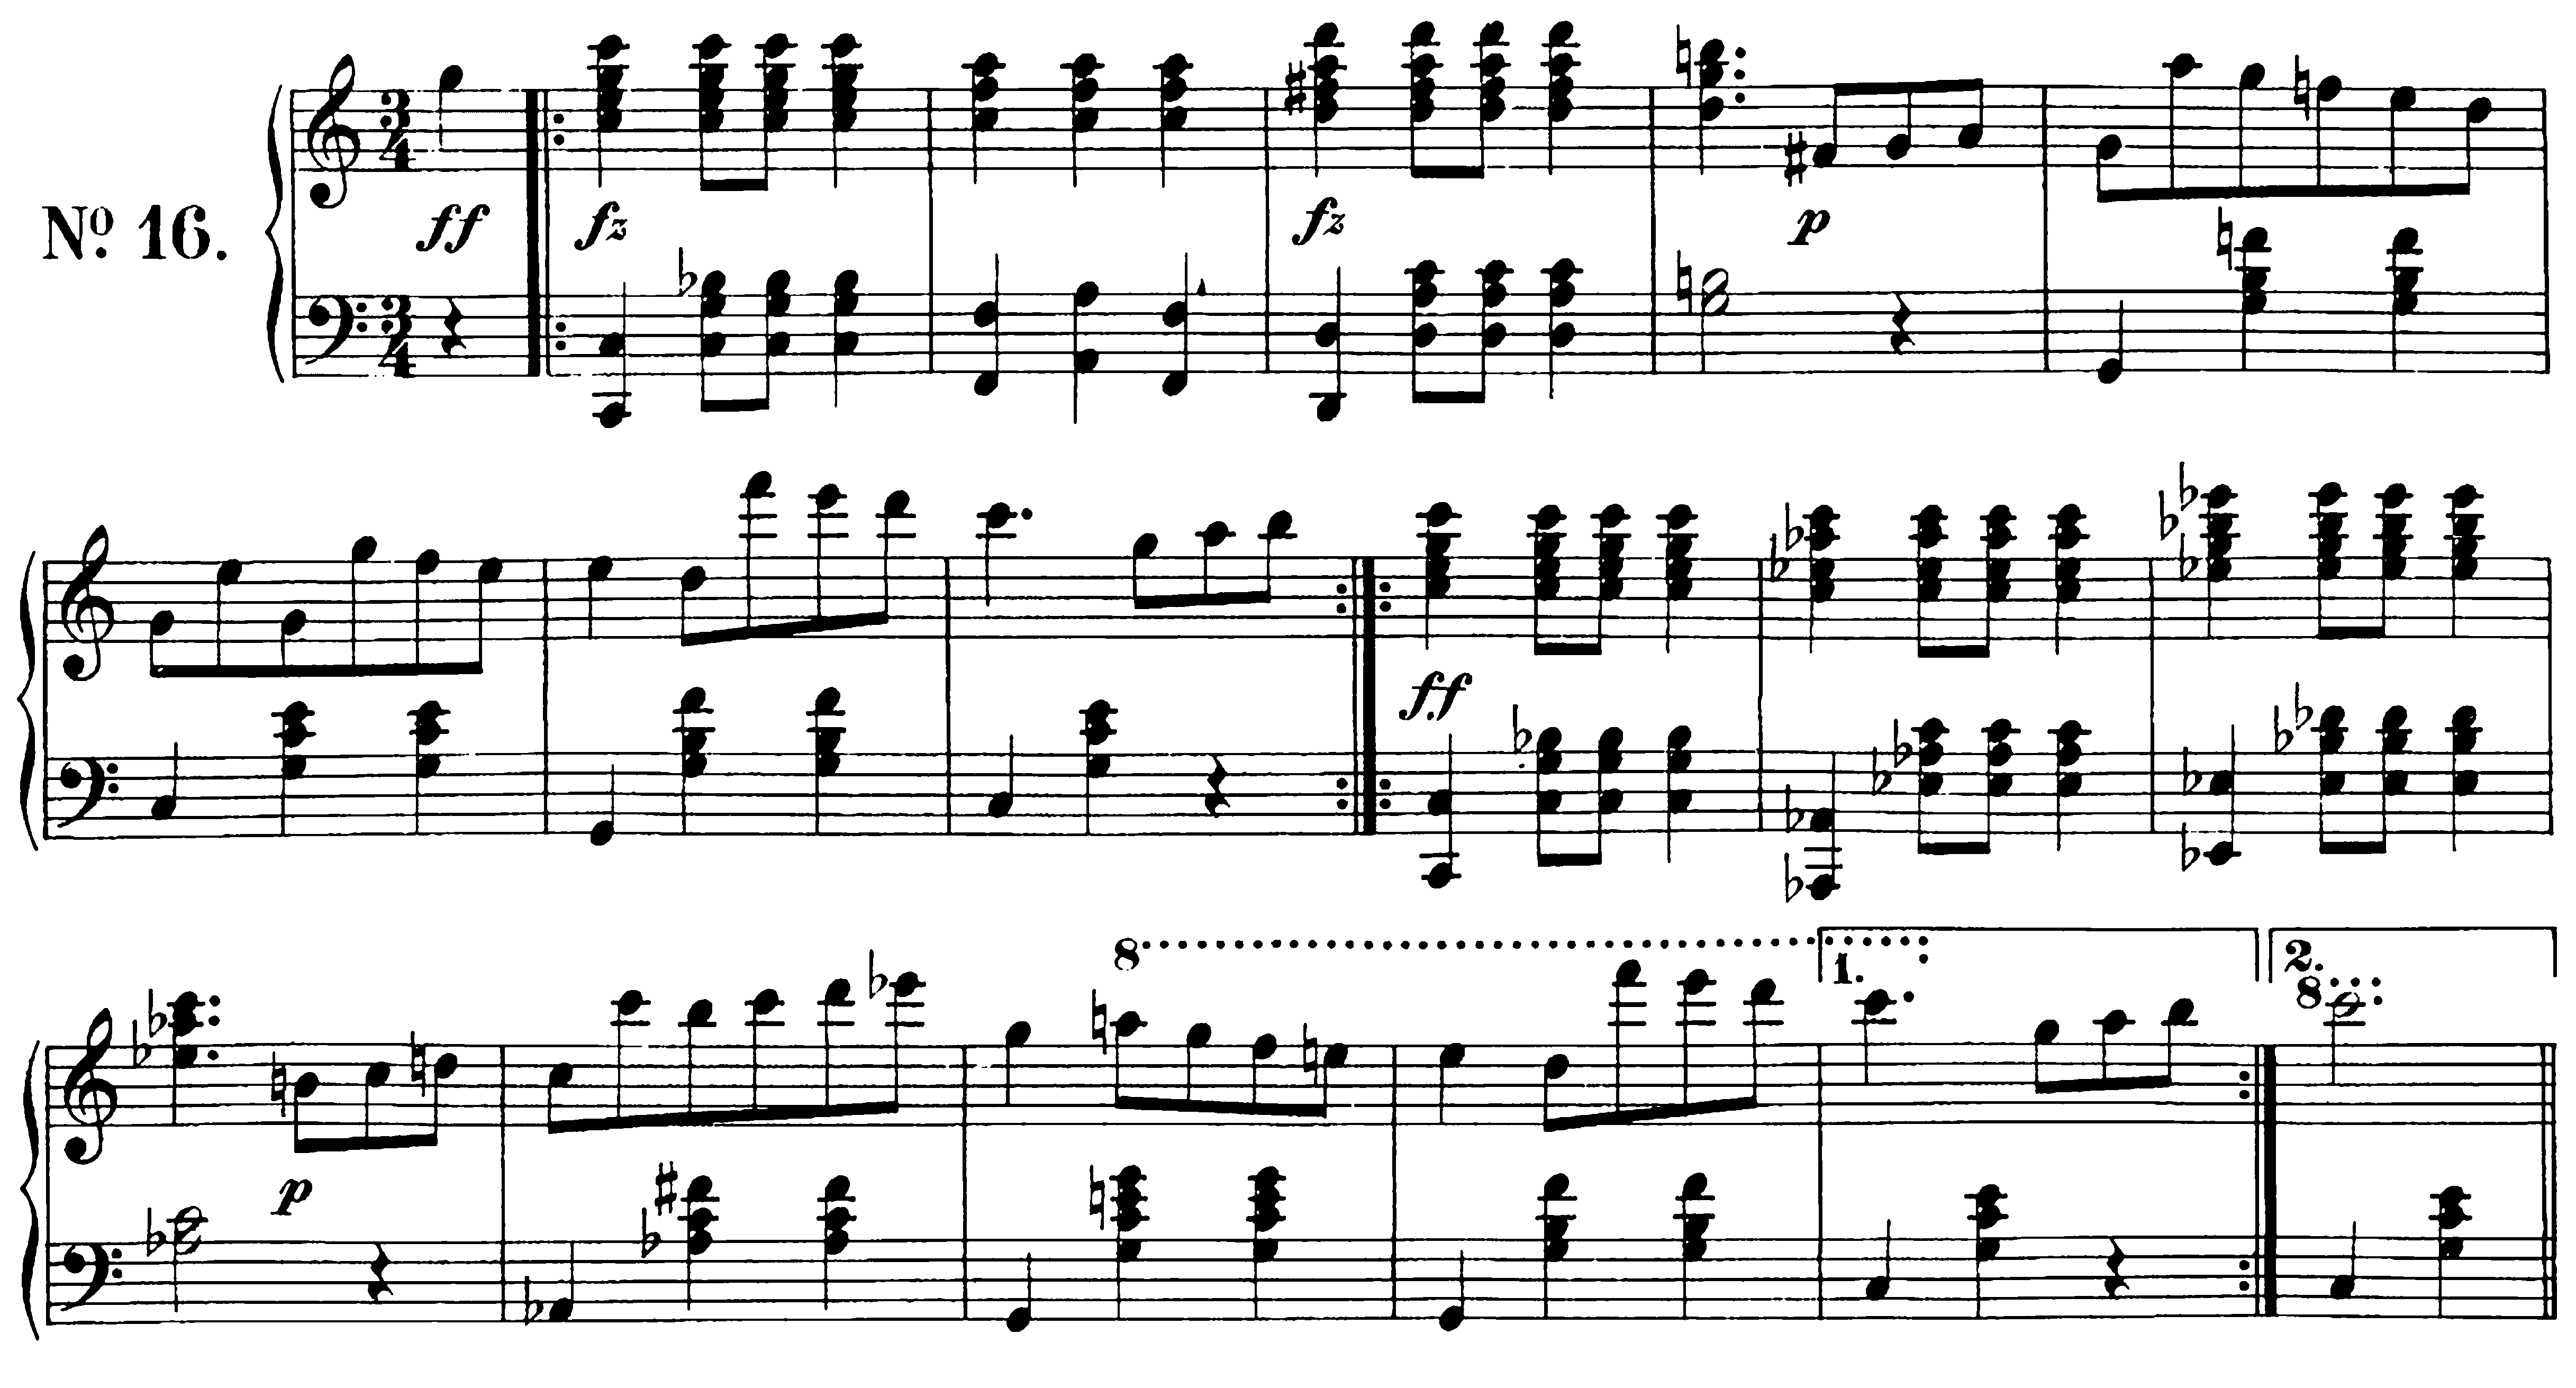
\includegraphics[width=1\textwidth]{figures/LitreatureReview/score2.png}
        \caption{}
        \label{fig:score}
    \end{subfigure}
    
    \caption[Example of symbol holding documents]{Different types of documents in which symbols are found such as (a) Electric schematics\footnotemark, (b) topographical map\footnotemark, (c) musical scores\footnotemark.}
    \label{fig:documentexamples}
\end{figure*}

\vspace{19mm}
\footnotetext[1]{Taken From \url{http://www.redcircuits.com/Page8.htm}}
\footnotetext[2]{Taken From \url{http://en.wikipedia.org/wiki/File:Topographic_map_example.png}}
\footnotetext[3]{Taken From \url{http://music.unt.edu/mhte/theory/TF}}


\section{Symbol Recognition}
Information is shared in many forms. It is often represented by textual or graphical means. At the core of human learning, lies the ability of pattern recognition and inference. This ability helps us to process information in any form it is presented, be it textual, graphical or otherwise. \\

In Artificial Intelligence (AI) research a constant effort is being put forward in order to model and automate these abilities by mechanical means \cite{duin2007science}. 
The successful modelling of such abilities yield various advantages. As described in Section \ref{sec:background}, such advantages include the automatic conversion of paper-based information into a equivalently meaningful digital version. This results in more convenient, efficient retrieval and manipulation of the information in question. In various fields, such as architecture, electronics, cartography, etc, information is conveyed in a diagrammatic form \cite{Llados}. Symbols constitute an important informative source in diagrams \cite{XML} and depending on the field and the application being used, different symbols can be found.  These symbols can be designed according to domain dependent rules or none at all. \\

This problem is tackled through symbol recognition. Symbol recognition is a field within pattern recognition area to which a lot of research effort has been devoted \cite{musings}. It is the automatic process where an input image of unknown pattern is classified to a particular class in a particular domain. \cite{Llados} \cite{luqman_2009}. This process is then used in the conversion of paper based graphical symbols into equivalent digital representations.\\

The process of symbol recognition can be divided into two main parts namely segmentation and recognition. The first part, segmentation of the document or image, is a prerequisite to the second part, recognition. Segmentation isolates the symbols from the document or image, for an easier and computationally lighter recognition process.\\

Combining segmentation and recognition into one system is one of the main problems within the field of symbol recognition. This problem is known as the "segmentation/recognition paradigm" \cite{delal2}. This problem describes that a document or image should be segmented before recognition can take place. However, at the same time, some kind of recognition needs to be applied for segmentation to take place \cite{yoon2001new}. \\

An other pre-requisite is that a system needs some priori knowledge about the symbols it needs to recognise in order to successfully recognise symbols \cite{delal2}. This corresponds to learning a database of model symbols for training purposes. Various shape recognition methods have been applied for this training phase. \\

Symbol recognition can be classified into two main categories, statistical and structural. Structural symbol recognition is based on the organisation of primitives, such as straight lines and arcs, into higher defined structures such as symbols or signatures \cite{ogierRobustSymbolRecognition}. On the other hand statistical symbol recognition is based on representing the symbol in simpler forms by the use of a shape descriptor \cite{Llados}. The following sub sections explain those two categories in detail.


\subsection{Statistical Symbol Recognition}
In a statistical approach towards symbol recognition, each symbol is represented by a unique signature. This signature is in the form of a feature vector of $n$ dimensions extracted from the same symbol. This approach has two important issues. The first issue is the selection of features for every pattern and the second one is the partitioning of the feature space \cite{Llados}. In this case, the feature space refers to the set of model symbols available.\\

The feature vector for every symbol is constructed depending on the properties of the inputted pattern. The chosen set of features for each symbol must be unique. This is critical to attain high discrimination power thus ultimately avoiding confusion between symbols in the classification process \cite{Llados}.\\

There are various methods with which a set of features is extracted from a pattern or symbols such as: centroids, line intersections, projection profiles, etc, amongst many \cite{Llados}. These methods adopt an invariant approach towards added noise, geometrical image transformations and distortions \cite{Llados}.Once that a set of features is chosen for each symbol, classification consists in choosing a segmentation method in order to partition the feature space. This is done on order to assign each feature vector to one of the available classes. \\

One of the simplest feature spaces is the image space it self, where the feature vector is composed of features each corresponding to a pixel with in the image. When an image is used as a feature space it is usually normalised to a certain size \cite{Llados}. Although this is one of the simplest feature spaces to process it has a number of advantages. It is simpler to process due to its low complexity, moreover it corresponds directly to the input information's visual appearance. However, it also has a number of disadvantages. This feature space does not adhere to an intravariant approach, therefore it does not take into consideration image distortion or geometrical transformations. Furthermore, it is very sensitive to noise. \\

The simplest way to partition a feature space consists in defining a distance function among the available feature vectors. This can be done by using the k-nearest neighbour algorithm (KNN). Which distance function to use in the Knn algorithm, depends on the application. One of the most popularly used distance functions is the Euclidean distance. The KNN algorithm is based on the concept of similarity \cite{Llados}. It takes into account the nearest $K$ number of neighbours which can weight in, in the classification of the presented pattern. Other methods have also been used for the classification of unknown patterns which are also based on the concept of similarity such as neural networks \cite{ANNS} and decision trees \cite{decisiontrees}.\\

Artificial neural networks (ANNs) have been proven to be adequate for classification purposes often achieving good recognition rates across various domains. One of the advantages in ANNs is their learning capabilities. They adapt quickly to the properties of the provided training set \cite{Llados}. \\

Decision trees for the purpose of symbol recognition are constructed in such a way that each of node in the tree corresponds to a particular feature. Classification is then carried out by visiting the nodes which satisfy a condition with the inputted image. This approach follows the tree branches which ultimately lead to a leave node which corresponds to a recognised symbol \cite{Llados}. \\

The main goal is to minimise, as much as possible, the distance between the input pattern and the pattern class it belongs to. At the same time, the distance between the same input pattern and other pattern classes is maximised \cite{Llados}.

\subsection{Structural Symbol Recognition}
In the structural approach towards symbol recognition, symbols are represented by a description of their shape in terms of simpler parts and the relationship between them \cite{Llados}. These parts are geometric primitives \cite{zernike} which usually consist of straight lines and arcs. However other geometric primitives have been also used such as loops, contours or simple shapes such as circles, rectangles etc. \\

Since the symbol is described by the geometric primitives it contains, a previous vectorization step is required. Vectorization is the process by which a raster image is converted into a set of geometrical primitives described above. Vectorization of raster images introduces both noise and distortion in the symbol's representation\cite{Llados}. \\

As cited in \cite{Llados} there is a large body of work about structural approaches focusing on symbol graph representation \cite{Groen, hamada, mediangraph,combi,graphmatch,engdrawings,1997combining}. When representing a symbol with a graph, each node and edge correspond to points and lines within the image. This provides a natural and intuitive symbol description. Classification for these methods consist in finding the best matching subgraphs between the input symbol and the models of the symbols. One of the main drawbacks for this method is its computational complexity. However some ways of reducing computation have been explored \cite{Llados}.\\

An other method of symbol representation in various structural approaches is by defining formal grammars. Graph grammars are the most common because of bi-dimensional structure of symbols \cite{Llados}. A grammar stores in a very compact manner all valid instances of a symbol or a class of symbols. Correct classification then consists of parsing its representation in order to test whether it can be generated by defined grammar. Grammars are useful in applications where the shape of the symbols can be accurately defined by a set of rules, for example technical drawings.\\

An other method which has also been used in structural approaches is the use of Hidden Markov Models (HMMs). HMMs is a powerful statistical tool for modelling generative sequences \cite{markovs}. HMMs are used since the structure of the symbol can be described as a sequence of states which generate the image. Recognition then consists in finding the sequence of states with the higher probability.

\subsection{Performance Evaluation}
\label{sec:perf}
During the last decade, attention has been shifted in the development of a generic and standard framework which permits the comparison and performance evaluation of symbol recognition methods. This effort has resulted in various contests such as the GREC contests taking place  which focus on the recognition of isolated symbols and thus creating a framework for evaluation reasons \cite{Delalandre_2012}.

\subsubsection{Datasets}
    
For the evaluation and comparison of the methods used in these contests, publicly available data sets of isolated symbols are generated \cite{Delalandre_contest} \cite{Delalandre_sketched}. These datasets are generated with a set of goals in mind \cite{Delalandre_contest}:

   \begin{enumerate}
        \item To provide a set of tests that could evaluate scalability of methods.
        \item To be able to test the performance of methods under some realistic increasing depredations.
        \item  To be able to test the generalisation ability of the methods.
    \end{enumerate}

The generated data sets are organised into four categories which have different levels of complexity due to noise, deformation, rotation and scaling. The first category consists of 24 data sets. Each data set contains a number (varying between 25 and 150) of different electrical and architectural symbols each represented by a single image. These data sets contain 1000 test images of deformed symbols of increasing complexity. For instance, the least complex data set contains images that are only slightly deformed, while the most complex data set consists of images of symbols with the highest deformation.\\

The second category consists of 3 datasets each having 150 different symbols. These datasets contain test symbols with geometrical transformation applied such as scaling, rotation or combined. The third category of datasets consists of 3 datasets each comprising of 150 different models as well with three different kinds of noise applied separately. \\

The method used to apply noise to the test images was proposed by Kanungo \cite{888707}. The remaining data sets contain images of geometrically transformed symbols, such as different orientations and scale. Fig. \ref{fig:noises} shows a sample of the test images with noise applied.

\begin{figure*}[h]
        \centering
        \fbox{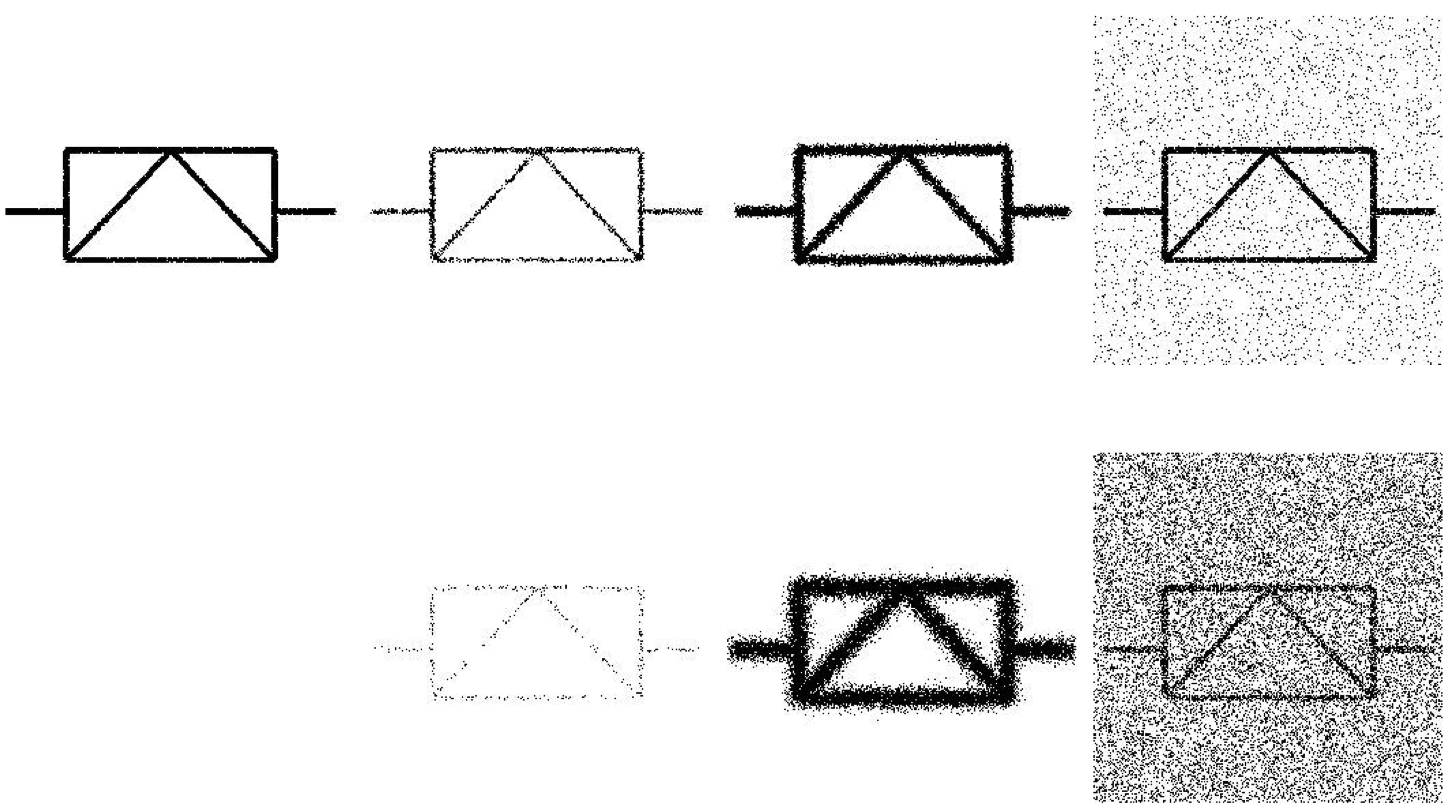
\includegraphics[width=0.5\textwidth]{figures/LitreatureReview/noises.png}}
        \caption[Sample test images which include noise]{A sample set of test images for the model, found at the top left corner of the image, with noise applied according to Kanungo's method \cite{888707}. Adapted from \cite{Delalandre_contest}.}
        \label{fig:noises}
\end{figure*}

The last, fourth, category contains three data sets. They contain large number of different model symbols and large number of test images that combine different degradation levels and different transformations \cite{Delalandre_2012}.

\subsubsection{Performance Metrics}
For the symbol recognition contest the chosen performance metric was the recognition rate \cite{Delalandre_2012}. The recognition rate is determined by counting the true positives (TP) and the false positives (FP). The recognition rate is then calculated as follows, where $R$ is the recognition rate in percentage.

\begin{equation}
    R = \left(\frac{1}{(TP+FP)} \times TP\right) \times 100
\end{equation}

\subsubsection{Results}
The authors report that only one participant submitted a method which approached both symbol spotting and recognition \cite{Nayef}. Amongst the global results reported, the following results are the ones attained by testing the second and third category of datasets. For each kind of deformation and noise a different result was attained. \\

\begin{table}[h]
\centering
\caption{Contest's results for the second category of datasets.}
\begin{tabular}{ccccccccccccccc}
  \hline
      Degradation & & & & & & & & Recognition Rate \\
  \hline
      Rotation & & & & & & & &  81.07 \% \\
      Scaling & & & & & & & &  89.20 \% \\
      RotationScaling & & & & & & & &  84.27 \% \\   
  \hline
\end{tabular}
\end{table}


\begin{table}[h]
\centering
\caption{Contest's results for the third category of datasets.}
\begin{tabular}{ccccccccccccccc}
  \hline
      Degradation & & & & & & & & Recognition Rate \\
  \hline
      Noise A & & & & & & & &  88.07 \% \\
      Noise B & & & & & & & &  85.73 \% \\
      Noise E & & & & & & & &  85.67 \% \\   
  \hline
\end{tabular}
\end{table}
      

The authors think that the datasets used in their work, can serve future similar contests as a stable platform against which evaluation and comparison  of symbol recognition methods can be done. Future editions will hold hand drawn symbols \cite{Delalandre_2012}.


\section {State of The Art}

Shape descriptors have been used in a variety of applications and tasks such as shape analysis, comparison and retrieval \cite{Heider}. In symbol recognition, as previously described, shape descriptors are an integral part of the process. The goal of the shape descriptor is to represent a pattern by a unique structure which relies on the extraction of local or global features. \\

As observed in previous studies \cite{Alajlan}, shape descriptors can be either global or local. Global shape descriptors take into consideration the entire shape of the object while local shape descriptors are used for local shape features \cite{wang}.Shape descriptors which are either global or local may fail to be robust. Global descriptors are reported to be robust to local deformations, but fail when trying to capture local shape details. At the same time local descriptors are adequate in representing local shape features, however they are very sensitive to noise \cite{wang}. \\

One of the most important challenges in shape descriptors is to come up with a solution by defining a rich shape descriptor, which consists of both Global and local properties. This solution needs to be computationally fast and efficient, compact, and most importantly, general enough to be used in a variety of applications.

The features that a shape descriptor detects represent information about specific structures within the image or pattern itself. This information ranges from simple geometric primitives such as point or edges to much more complex ones such as objects or a set of primitives. The extraction of such features is a very critical problem in computer vision and is used widely in various vision related tasks such as object recognition and tracking \cite{Maji_comparison}. Due to their importance, a lot of research attention has been dedicated to it \cite{Heider, Maji_comparison}. \\

Depending on the application an intravariant approach towards feature extraction becomes important. One of the most important jobs of a shape descriptor is to extract unique features which are both repeatable as well as invariant to various conditions such as noise or distortion. Apart from this a good shape descriptor should be informative, discriminative and efficient in matching process \cite{wang}. The rest of this section reviews a number of feature descriptors applied to date. \\

A very popular shape descriptor is the Shape Context approach. It is feature descriptor which was proposed by S. Belongie and J. Malik in 2000 \cite{context}. Given a collection of points within an image which have been extracted from a set of detected edge elements, the shape context descriptor captures the relative distribution of points in the plane relative to each point on the shape \cite{contextWeb}. \\

A very popular shape descriptor is the Shape Context approach. It is feature descriptor which was proposed by S. Belongie and J. Malik in 2000 \cite{context}. Given a collection of points within an image which have been extracted from a set of detected edge elements, the shape context descriptor "captures the relative distribution of points in the plane relative to each point on the shape" \cite{contextWeb}. \\

The shape context approach operates on the concept of similarity where it is measured between shapes and exploited for pattern recognition purposes. For example, when taking into account two written digits, Fig \ref{fig:similarity}, interpretation can differ. When taken as a set of pixel with various brightness values, the two digits are very different. However when observed by a human, they appear to be very similar.


\begin{figure*}[h]
        \centering
        \fbox{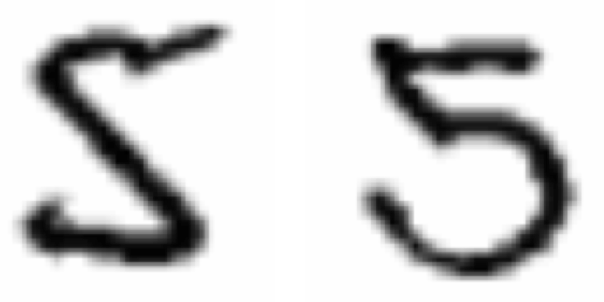
\includegraphics[width=0.2\textwidth]{figures/LitreatureReview/similiar.png}}
        \caption[An example of similarity]{Two written digits can be interpreted differently depending who the observer is. Adapted from \cite{context}.}
        \label{fig:similarity}
\end{figure*}

The aim of the authors is to put into operation the concept of similarity for object classification. This approach is described as a three stage process \cite{context}:

\begin{enumerate}
    \item "Solve the correspondence problem between the two shapes"
    \item "Use the correspondences to estimate an aligning transform"
    \item "Compute the distance between the two shapes as a sum of matching errors between corresponding points, together with a term measuring the magnitude of the aligning transformation"
\end{enumerate}

At the core of the similarity concept that the authors use in their work is the fact that it has been observed that shapes which are related but not identical, can often be deformed to a point where they are aligned using simple coordinate transformations, Fig. \ref{fig:fish}. Therefore, based on this the authors have come up with an algorithm which finds correspondences between similar shapes. \\

\begin{figure*}[h]
        \centering
        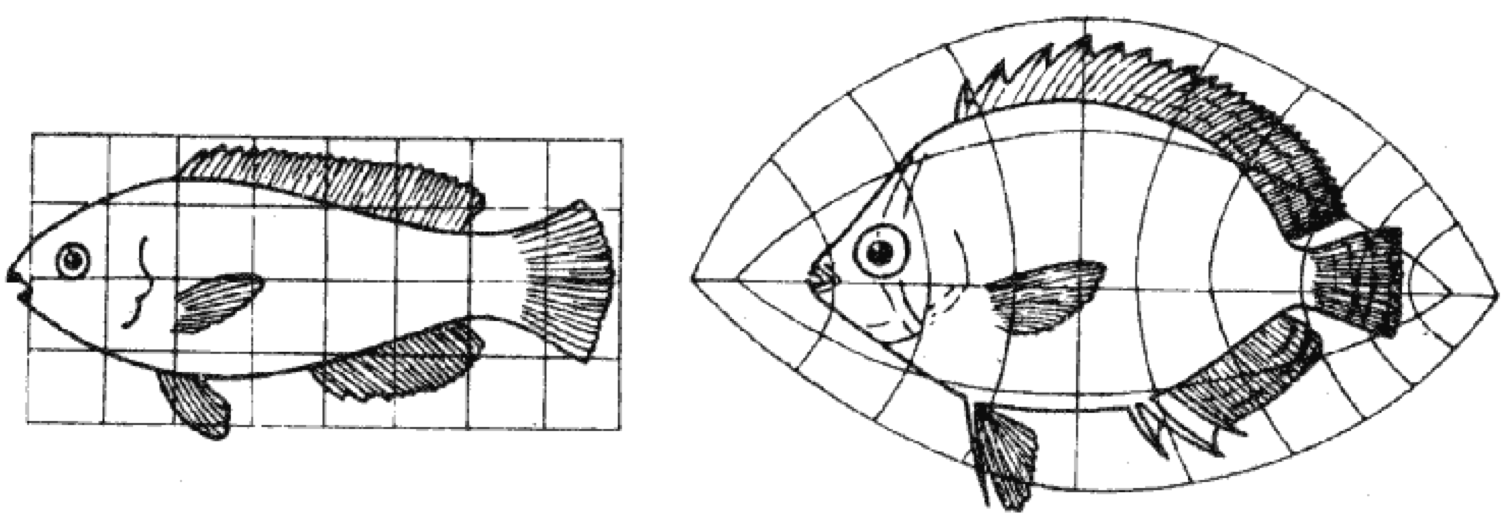
\includegraphics[width=0.9\textwidth]{figures/LitreatureReview/fish.png}
        \caption[An example of simple coordinate transformations between similar objects]{An example of coordinate transformation between two similar objects. Adapted from \cite{context}.}
        \label{fig:fish}
\end{figure*}

In this approach, shapes are represented by a collection of points. This collection of $n$ number of points is sampled from the shape's contours by using an edge detector. When these points are taken into consideration on their own, they hold no particular importance.\\

\begin{figure*}[h]
        \centering
        \begin{subfigure}[b]{0.36\textwidth}
                \centering
                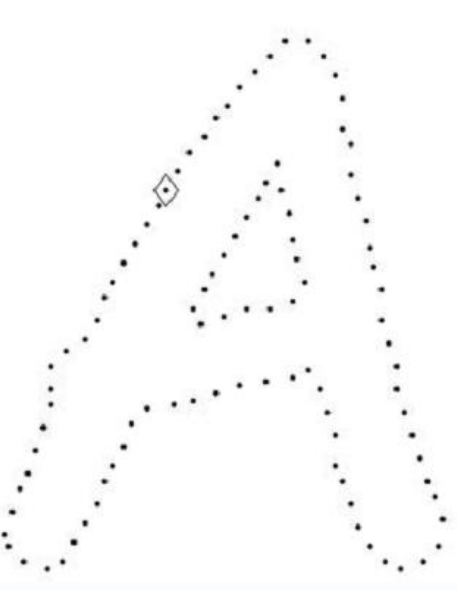
\includegraphics[width=0.6\textwidth]{figures/LitreatureReview/letter.png}
                \caption{}
        \end{subfigure}
        \begin{subfigure}[b]{0.36\textwidth}
                \centering
                \includegraphics[width=0.7\textwidth]{figures/LitreatureReview/letterpoints.png}
                \caption{}
        \end{subfigure}
        \caption[Point selection and calculated distribution shape context descriptor]{(a) A point is selected from a collection of points representing the shape. (b) Using a diagram of log-polar histogram bins we compute the point distribution and thus the shape contexts. Adapted from \cite{context}.}
        \label{fig:contextPart1}
\end{figure*} 

The shape context descriptor then describes the distribution of the rest of the shape relative to a selected point by placing a diagram of log-polar histogram bins on the selected point, Fig. \ref{fig:contextPart1}. The histogram is divided into a number of bins. From each of these bins the number of points is counted. This will describe the spatial arrangement of point around the selected point. When the selected shape needs to be matched to an other shape, the same procedure is applied to the other shape. Once this is done the arrangement attained from one shape is compared to the other one. Fig. \ref{fig:contextPart2} shows two different shapes of similar shape. From each a point has been chosen to check for correspondence between the two shapes.\\ 

\begin{figure*}[h]
        \centering
        \begin{subfigure}[b]{0.36\textwidth}
                \centering
                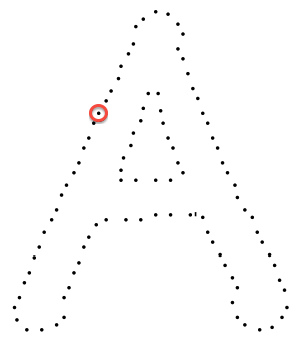
\includegraphics[width=0.7\textwidth]{figures/LitreatureReview/lettera.png}
                \caption{}
                \label{fig:lettA}
        \end{subfigure}
        \begin{subfigure}[b]{0.36\textwidth}
                \centering
                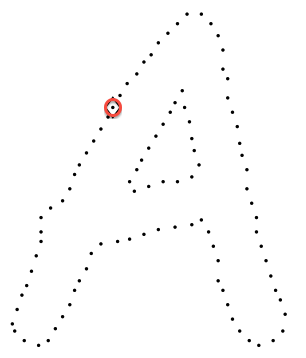
\includegraphics[width=0.7\textwidth]{figures/LitreatureReview/letterb.png}
                \caption{}
                \label{fig:lettB}
        \end{subfigure}
        \caption[Choice of points from two similar shapes for calculation of shape context]{(a) A Point is selected from a shape to be compared to (b) an other point from a similar shape. Adapted from \cite{context}.}
        \label{fig:contextPart2}
\end{figure*}

For each point a shape context is calculated as a log-polar histogram of the coordinates of the rest of the collection of points using the selected point as the origin, Fig. \ref{fig:contextPart3}.\\

\begin{figure*}[h]
        \centering
        \begin{subfigure}[b]{0.36\textwidth}
                \centering
                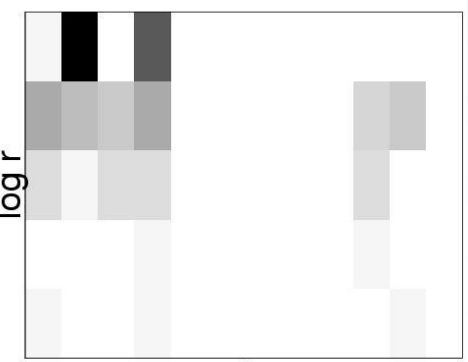
\includegraphics[width=0.7\textwidth]{figures/LitreatureReview/responsea.png}
                \caption{}
        \end{subfigure}
        \begin{subfigure}[b]{0.36\textwidth}
                \centering
                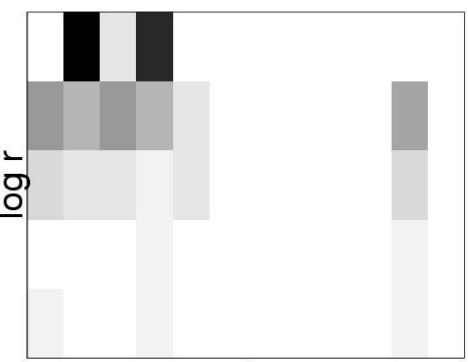
\includegraphics[width=0.7\textwidth]{figures/LitreatureReview/responseb.png}
                \caption{}
        \end{subfigure}
        \caption[Shape context result for two points from two similar shapes]{(a) Shows the shape context response for the point in Fig.\ref{fig:lettA}. While (b) shows the shape context response for the point in Fig.\ref{fig:lettB}. Adapted from \cite{context}.}
        \label{fig:contextPart3}
\end{figure*}



After the responses have been attained, the correspondences are found. This means that for each sample point on the first shape, a sample point of the most similar context is found on the second shape. The correspondence is then extended by an estimation of transformation alignment that maps one shape onto the other, Fig. \ref{fig:contextResult}.

\begin{figure*}[h]
        \centering
        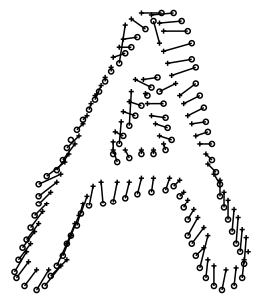
\includegraphics[width=0.3\textwidth]{figures/LitreatureReview/contextResult.png}
        \caption[Estimated transformation alignment between two shapes in shape context]{The difference between the two shapes. Adapted from \cite{context}.}
        \label{fig:contextResult}
\end{figure*}

Once this has been attained, and the similarity can be measured, a nearest neighbour technique can be used for recognition. Object recognition using shape context as a descriptor has been used in a variety of applications. The authors present results on the MNIST dataset of handwritten digits, silhouettes, line drawings, and CAPTCHA images \cite{context}.\\

Another recently proposed approach to build a shape descriptor is by the use of height functions, proposed in \cite{wang}. In this approach each object is represented by a contour. This contour is made up of a fixed finite number of sample points. For each of those sample points, a height function is defined based on the distances of the other sample points to its tangent lines. The height function is defined as a vector of distances of the other sample points to its tangent line. \\

Once these height functions are obtained a process called smoothing is performed on them. This makes the descriptor more compact and insensitive to local deformations. Ultimately, the shape of an object is represented as a sequence of the height functions \cite{wang}. The proposed descriptor is reported to be invariant to geometric transformation and also insensitive to deformations due to noise or occlusion. \\

The process starts by defining the contour of the shape. Once this contour is defined a collection of equidistant points are set on it. This set of points is denoted as $X = \{x_{i}\ (i=1,...,N)\}$ where $N=100$. Once that those sample points have been set an other important step before the calculation of height functions is to determine the axes.\\ 

Previously (Liu et al., 2008), height values were computed in a number of different directions. This however resulted into very high time complexity. Instead, the authors adjusted the angular direction for each of the selected points. In their work, the authors observe that a tangent line is an excellent reference line for height functions. The tangent line, $l_{i}$, for each sample point,$x_{i}$, is defined according to the contour orientation. Therefore the tangent line is starts from $x_{i-1}$ and goes to $x_{i+1}$. \\

Then the distance between an other point, $x_{j}$, and the tangent line $l_{i}$ is defined as height value $h_{ij}$. According to which side $x_{j}$ resides a value is assigned. If it is to the left of the tangent line the value is positive, if to the right the value is negative and of the point is just on the axis of the tangent line, the value is zero. The authors point out that if the height value is more precise if its value is positive or negative. That way we can know on which side the point relies. Fig. \ref{fig:heightfunc} shows an example of this process where the height functions for point $x_{i}$ are calculated.\\

\begin{figure*}[h]
        \centering
        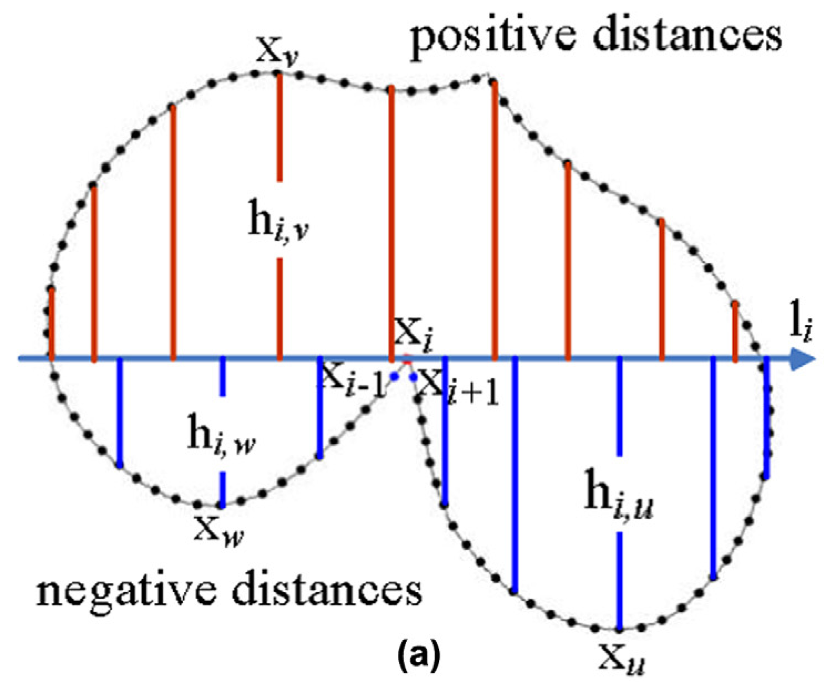
\includegraphics[width=0.7\textwidth]{figures/LitreatureReview/heightfunc.png}
        \caption[Example of height functions.]{(a) Example of height functions being calculated according to sample point $x_{i}$. Adapted from \cite{wang}.}
        \label{fig:heightfunc}
\end{figure*}

In Fig. \ref{fig:heightfunc}, the height functions for $x_{i}$ are being calculated. The tangent line $l{i}$ is defined by using $x_{i-1}$ and $x_{i+1}$. In this case, the tangent line is a horizontal one. Then the distance between other points and the tangent line is calculated. For instance, from point $x_{u}$ to tangent line $l_{i}$, the height value is $h_{i,u}$. Upon doing so we can determine on which side of the tangent line the calculated points lie. For instance $h_{i,y}$ has a positive value and therefore its corresponding point,$x_{y}$,lies to the left of the tangent line, while $h_{i,w}$ and $h_{i,u}$ have negative values therefore points $x_{u}$ and $x_{w}$ lie on the right of the tangent line. This is done for each of the sample points, their height value is calculated according to tangent line $l_{i}$. And the shape descriptor for point $x_{i}$ with respective to the shape X is the ordered sequence of the height values. \\

The development of efficient and robust shape descriptors is a topic of on going research. Apart from the ones described in this section are various other techniques have been developed \cite{descriptor1,descriptor2,descriptor3,descriptor4,descriptor5}.

\section{COSFIRE Filters}
COSFIRE filters are effective for key point detection and pattern recognition. They are trainable because they can be configured with any given prototypes. They are constructed by a configuration process which automatically analyses the dominant orientations and their mutual spatial arrangement of a given prototype pattern of interest \cite{Azzopardi_Petkov_2012}. We use Gabor filters to detect the dominant orientations. The response of a COSFIRE filter is computed as the weighted geometric mean of the involved Gabor filter responses. This means that a response is only achieved when all the concerned contour parts are present \cite{Azzopardi_Petkov_2012}.

\subsubsection {Gabor Filters}
A one dimensional Gabor function is defined as the multiplication of a sinusoid with a Gaussian window as shown Fig. \ref{fig:1DGabor}. Gabor functions have then been extended to two-dimensions, as the product of an elliptical Gaussian and a sinusoid plane wave \cite{Daugman1985}. Fig. \ref{fig:2DGabor} illustrates a Gabor function map that is tuned for vertical bars.

\begin{figure*}[h]
        \centering
        \begin{subfigure}[b]{0.3\textwidth}
                \centering
                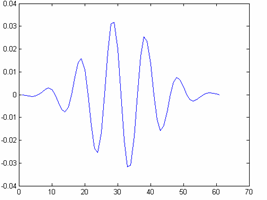
\includegraphics[width=1.0\textwidth]{figures/LitreatureReview/GaborFunction.png}
                \caption{Gabor Function}
                \label{fig:gabor}
        \end{subfigure}
        \begin{subfigure}[b]{0.3\textwidth}
                \centering
                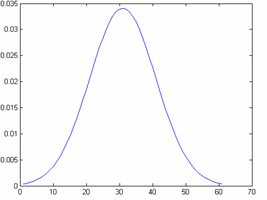
\includegraphics[width=1.0\textwidth]{figures/LitreatureReview/GaussianFunction.png}
                \caption{Gaussian Function}
                \label{fig:gaus}
        \end{subfigure}
        \begin{subfigure}[b]{0.3\textwidth}
                \centering
                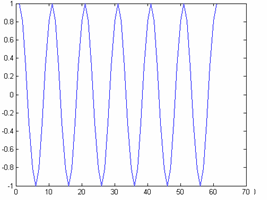
\includegraphics[width=1.0\textwidth]{figures/LitreatureReview/CosineFunction.png}
                \caption{Cosine Function}
                \label{fig:gaus}
        \end{subfigure}
        \caption[Example of a 1D Gabor Function]{(a) A one dimensional Gabor function is the product of a (b) Gaussian function and a (c) cosine function.}
        \label{fig:1DGabor}
\end{figure*}

\begin{figure*}[h]
        \centering
        \begin{subfigure}[b]{0.3\textwidth}
                \centering
                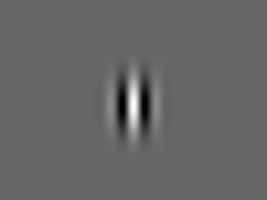
\includegraphics[width=1.0\textwidth]{figures/LitreatureReview/GaborFunction2D.png}
                \caption{Gabor Function}
                \label{fig:gabor}
        \end{subfigure}
        \begin{subfigure}[b]{0.3\textwidth}
                \centering
                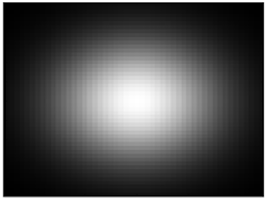
\includegraphics[width=1.0\textwidth]{figures/LitreatureReview/GaussianFunction2D.png}
                \caption{Gaussian Function}
                \label{fig:gaus}
        \end{subfigure}
        \begin{subfigure}[b]{0.3\textwidth}
                \centering
                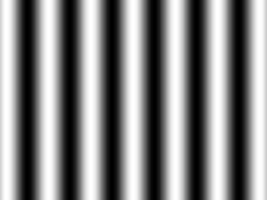
\includegraphics[width=1.0\textwidth]{figures/LitreatureReview/CosineFunction2D.png}
                \caption{Cosine Function}
                \label{fig:gaus}
        \end{subfigure}
        \caption[Example of a 2D Gabor Function]{(a) A two dimensional Gabor function is the product of an (b) elliptical Gaussian and a (c) complex plane wave.}
        \label{fig:2DGabor}
\end{figure*}

In their research Jones and Palmer \cite{JonesPalmer1987} demonstrated that two dimensional (2D) Gabor functions, which were proposed by Daugman \cite{Daugman1985}, can be used to model receptive fields of the orientation- selective simple cells of cats. Fig. \ref{fig:CatReceptiveField} shows the similarity between two dimensional Gabor functions and receptive fields of cats’ simple cells. The top row shows 2D receptive field profiles while the second row shows their corresponding best fitting Gabor functions \cite{Daugman1988}. \\


Daugman’s research \cite{Daugman1985} enabled the use of Gabor functions in computer vision applications as means to analyse images \cite{Daugman1988}. Recently, a novel CORF (Combination of Receptive Fields) computational model was proposed in \cite{CORF_2012}. The authors demonstrated that the CORF model exhibits more properties that are typical of simple cells than the Gabor function model. The CORF model also achieves better performance in contour detection tasks.


\begin{figure}[t]
        \centering
        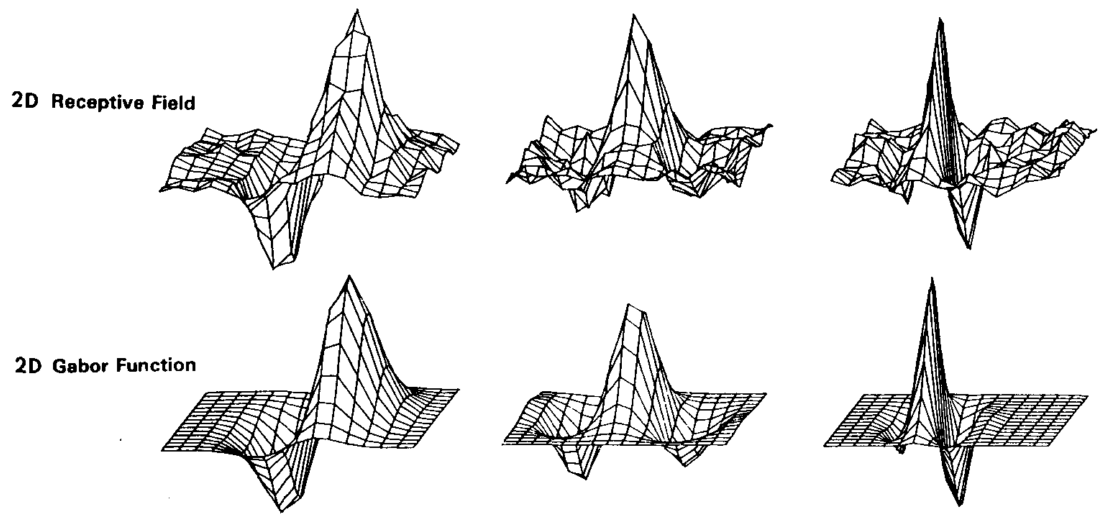
\includegraphics[width=1\textwidth]{figures/LitreatureReview/CatReceptiveFields.png}
        \caption[Receptive field profiles of some cells in cats visual cortex]{(First row) The receptive field profiles of some cells in a cat’s visual cortex compared to their corresponding best fitting (second row) two dimensional Gabor functions. Adapted from \cite{Daugman1988}.}
        \label{fig:CatReceptiveField}
\end{figure}


